%!TEX root = ../../main.tex
\begin{figure}[h]
    \centering
    \begin{subfigure}[b]{1\textwidth}
    \centering
    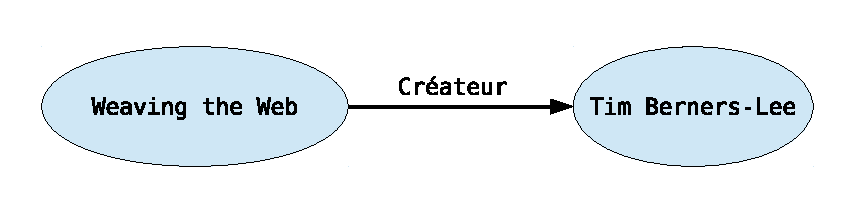
\includegraphics[width=0.85\textwidth]{figs/A/rdf-statement-example-graph.eps}
    \caption{Une illustaion graphique d'une assertion
      \acrshort{rdf}.}~\label{fig:rdf-statement-example-graph}
    \end{subfigure}

    \begin{subfigure}[b]{1\textwidth}
      \centering
      \lstinputlisting[language={XML}]{figs/A/rdf-statement-example.rdf}
      \caption{Une représentation
        \acrshort{rdf/xml}~\cite{beckett2004rdf} de l'assertion
        illustrée dans la
        figure~\ref{fig:rdf-statement-example-graph}.}~\label{fig:rdf-statement-example-xml}
    \end{subfigure}

    \caption{Un exemple d'une assertion
      \acrshort{rdf}.}~\label{fig:rdf-statement-example}
\end{figure}
%%% Local Variables:
%%% mode: latex
%%% TeX-master: "../../main"
%%% End:
